\section{About Microbenchmmarks}
A common practice to measure the performance of a fragment of code, or to compare it to the performance of some other code fragment is to create a micro benchmark. Throughout this document, there are multiple references to benchmarks of this kind, since their results helped us make decisions about how to best implement some specific library features.

A micro benchmark usually involves wrapping the code under evaluation inside a loop, to:

\begin{description}
\item[First] Be able to evalute the time it takes to perform the operation multiple times (a single execution could either be too small or an outlier and the measurement could have too much variance/error).
\item[Second] Allow JIT optimizations to kick in.
\end{description}

The first point is applicable to all programming languages but the second one is only important in engines/VMs that perform such optimizations. This document discusses the performance of JavaScript and in particular v8, so the second point does affect our benchmarks.

\subsection{A small example\protect\footnote{The example is based on \cite{mraleph-bc}.}}
Let's assume that we want to profile the following function:
\begin{lstlisting}[caption=Function to benchmark]
function between(a, b, c){
  return a <= b <= c;
}
\end{lstlisting}

A naive benchmark for it could be:
\begin{lstlisting}[caption=Naive benchmark]
// begin setup
function between(a, b, c){
  return a <= b && b <= c;
}
var a = Math.round(Math.random()*100);
var b = Math.round(Math.random()*100) + a;
var c = Math.round(Math.random()*100) + b;
//end setup
//start benchmark
console.time('between');
for (var i = 0; i < 100000; i++){
  between(a, b, c);
}
console.timeEnd('between');
//end benchmark
\end{lstlisting}

The problem with the above benchmark is that it does not consider optimizations. Let's assume that the executing engine is smart enough to:
\begin{enumerate}
  \item Inline functions
  \item Detect loop invariants
\end{enumerate}

Then due to \#1 the above could result in:
\begin{lstlisting}[caption=Naive benchmark after inlining]
// begin setup
var a = Math.round(Math.random()*100);
var b = Math.round(Math.random()*100) + a;
var c = Math.round(Math.random()*100) + b;
//end setup
//start benchmark
console.time('between');
for (var i = 0; i < 100000; i++){
  var j = a <= b && b <= c;
}
console.timeEnd('between');
//end benchmark
\end{lstlisting}

When it applies \#2, it realizes it does not need to perform the comparison in every iteration so it could extract it outside the loop, resulting in
\begin{lstlisting}[caption=Naive benchmark after evaluating loop invariants]
// begin setup
var a = Math.round(Math.random()*100);
var b = Math.round(Math.random()*100) + a;
var c = Math.round(Math.random()*100) + b;
//end setup
//start benchmark
console.time('between');
var j = a <= b && b <= c;
for (var i = 0; i < 100000; i++){
}
console.timeEnd('between');
//end benchmark
\end{lstlisting}

Alternatively it could notice that the variable \code{j} is not being used so it could just throw the line away. In any case, we would just be measuring how long it takes for JavaScript to execute the loop, which is not what we originally intended to do. To verify that is not the case the tool IRHydra\cite{ir-hydra} can be used , which \textit{can display intermediate representations used by V8}. As shown in the following figure, v8 inlined the function (the blue chevron marks that) but the loop invariant was not detected and optimized:
\begin{figure}[h!]
  \centering
  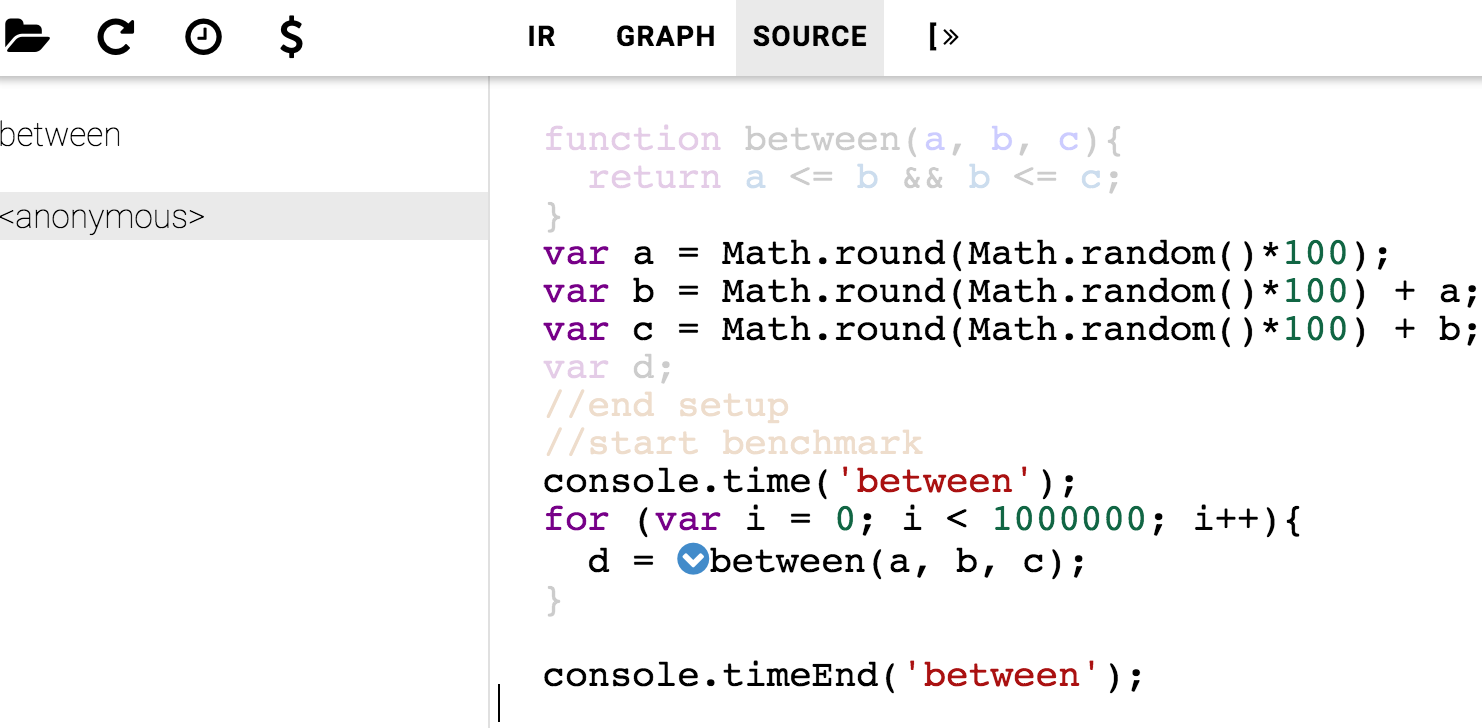
\includegraphics[width=1\textwidth]{naive_benchmark_ir_hydra}
  \caption{Optimized benchmark code with inlined function.}
\end{figure}

\subsection{Details}
\label{sub-sec:serialization-and-transference}
The benchmarks are executed using two different machines:

\textbf{Machine 1}
\begin{itemize}
  \item Mac Book Pro Retina
  \item Intel Core i7 2.8GHz
  \item 16 GB RAM DDR3 1600 MHz
  \item SSD 250 GB
  \item Chrome 41.0.2272
\end{itemize}

\textbf{Machine 2}
\begin{itemize}
  \item Mac Book Air
  \item Intel Core i5 1.8GHz
  \item 4 GB RAM DDR3 1600 MHz
  \item SSD 128 GB
  \item Chrome 40.0.2214
  \item Firefox Nightly 41.0a1
\end{itemize}

\note{Each benchmark is executed 5 (five) times to reduce variance.}

\note{No browser plug-ins are enabled when running the benchmarks as those could introduce additional sources of error.}
\pagebreak